\documentclass[12pt, twocolumn]{article}

\usepackage{biblatex}
\bibliography{\jobname}

%\usepackage[print]{3201report}
\usepackage{3201report}
\setboolean{shortarticle}{true}


\title{GAs To Solve The Travelling Salesman Problem}
\def\journalname{GAs To Solve The Travelling Salesman Problem}
\author{Jacob House, Nabil Miri, Omar Mohamed, and Hassan El-Khatib}
\dates{Compiled~\today\hfill\break Submitted~December~10,~2018}
\institution{Memorial University of Newfoundland, Faculty of Science, Department of Computer Science} 
\course{Computer Science 3201}

\begin{abstract}
	This report investigates the {\em Travelling Salesman Problem} through 
	the use of a genetic algorithm (GA) employing the {\em inver-over} 
	crossover operator, a combination of scramble and swap mutations, 
	and a combination of $\mu + \lambda$ and replacement survival 
	selection operators.
\end{abstract}


\begin{document}
	\maketitle
	\section{Problem Specifications}
	%% BREAK LINES EVERY 80 CHARACTERS TO HELP GIT WITH MERGING
Wolfram MathWorld defines the Travelling Salesman Problem (TSP) as ``a 
problem in graph theory requiring the most efficient (\ie least total distance) 
Hamiltonian cycle a salesman can take through each of $n$ cities,'' for which
``no general method of solution is known.'' \cite{tsp_wolfram_alpha} The 
website also remarks that the problem is assigned to the class of NP-hard 
(non-deterministic polynomial time) problems.

Given three datasets, for territories Western Sahara, Uruguay, and Canada of 
size $29$, $734$, and $4,663$ cities, respectively, the objective has been 
to design a genetic algorithm from scratch in the Python programming language
to solve the TSP for each locale using some advanced technique(s).

The first advanced technique employed in the algorithm is the {\em inver-over}
hybrid crossover/mutation operator. 




	\section{The Inver-Over Operator}
	%% BREAK LINES EVERY 80 CHARACTERS TO HELP GIT WITH MERGING
The inver-over operator can be regarded as either a crossover or mutation 
operator because it takes information from other individuals in the GA's
mating pool, yet bases a single offspring off of a single primary parent, much 
the same way a mutation operator is unary, performing mutation on a single
individual \cite{p44}. Throughout this report, the inver-over operator will 
be referenced as a crossover operator as this was the inver-over 
algorithm's place in the GA developed.

\subsection{Usefulness}
As {\em inver-over} embodies aspects of both crossover and mutation 
operators, the operator  is designed to provide middle-ground to 
algorithms relying primarily on crossover for variation (as this is 
computationally expensive) and those relying on mutation for variety,
since this is often ineffective in escaping local minima%
\footnote{Local minima occur when the natural selection in the GA 
	narrows the gene pool towards a ostensibly optimal solution and 
	eliminates individuals that otherwise would evolve to become the 
	true optimal solution.} \cite{p44}.


\subsection{Representation}
A set $P$ of individuals of length $n$, each represented as a sequence
\begin{equation*}
i_k = \langle C_{c_k(0)}, C_{c_k(1)}, C_{c_k(2)}, \ldots, C_{c_k(n-1)} \rangle\text{,}
\end{equation*}
where $c_k\colon \{0, 1, \ldots, n-1\} \to \{ 1, 2, \ldots, n \}$ is a bijection 
between indices of $i_k$, $0 \leqslant k < \card(P)$, and city indices as 
provided in the data file, is used to denote the population. Let 
$M \subsetneq P$ be the mating pool containing individuals 
$i_{m(0)}, i_{m(1)},\ldots, i_{m(\card(M)-1)}$ with $m\colon 
\{0, \ldots, \card(M)-1\} \to \{0, \ldots, \card(P) -1\}$
 an injective function mapping individuals in the mating pool $M$ to 
their equal `self' in the population $P$.

Fitness of an individual $i_k$, denoted by $\fit(i_k)$ in the Algorithm~\ref{alg:inver-over}, is then determined by the formula in 
\eqref{eq:fit1}.
\begin{equation}
\fit(i_m) = \sum_{j=0}^{n-1} \left\lVert \overrightarrow{C_j \, C_{j+1}} \right\rVert, \label{eq:fit1} 
\end{equation}
where 
\begin{equation*}
\left\lVert \overrightarrow{C_j \, C_{j+1}} \right\rVert = \sqrt{(x_{C_{j+1}} - x_{C_j})^2 + (y_{C_{j+1}} - y_{C_j})^2}
\end{equation*}
is the Eucliean distance between cities $C_j$ and $C_{j+1}$.\footnote{
	Take indices $j$ modulo $n$ so when $j=n-1$, $(n-1)+1  \equiv 0 \pmod n$
	 and we compute the distance from the last city back to the first.} Hence
a lower fitness score is better.

\subsection{Algorithm}
The algorithm (Algorithm~\ref{alg:inver-over}) used mirrors that 
depicted in the article by Tao and Michalewicz \cite{p44}.

\begin{algorithm}[H]
	\caption{The inver-over operator}\label{alg:inver-over}
	\small
	\begin{algorithmic}[1]
		\Require
		\Statex{$\triangleright$ $M$ be the mating pool}
		\Statex{$\triangleright$ \parbox[t]{0.9\linewidth}{$0 \leqslant i < \card(M)$ be the index of the initial parent}}
		\Statex{$\triangleright$ $n$ be the number of cities in the tour}
		\Ensure
		\Statex{$\triangleright$ New offspring individual created}
		\Statex
		\State{\textbf{var} $child := M[i]$} \Comment{Copy the parent}
		\State{\textbf{var} $unused := \{x \in \mathbb Z \mid 0 \leqslant x < n-1\}$} 
		\State{\textbf{var} $p := \frac{1}{2}$} 
		\State{\textbf{var} $c := \rand(unused)$} \Comment{Select randomly}
		\State{$unused  := unused\,\backslash\{c\}$}
		\While{$\card(unused) > 0$}
		\If{$\rand\{x \in \mathbb R \mid 0 \leqslant x < 1\} < p$}
		\State{$c' := \rand(unused)$}
		\Else
		\State{$newPar := \rand(M)$} 
		\State{$newParC := \where(newPar = child[c])$}
		\Statex \Comment{Index $j$ in $newPar$}
		\State{$c' := newParentC + 1$}
		\EndIf
		\State{$unused := unused\,\backslash\{c'\}$}
		\If{$child[c\pm1] = child[c']$}
		\State{\textbf{break} from the \textbf{while} loop}
		\EndIf
		\State{$child[c:c'] := child[c':c]$} \Comment{Invert}
		\State{$c := c'$}
		\EndWhile
		\If{$\fit(child) \geqslant \fit(M[i])$}
		\State{\textbf{return} $child$}
		\Else 
		\State{\textbf{return} $M[i]$}
		\EndIf 
	\end{algorithmic}
\end{algorithm}

Here $M[i]$ is the primary parent from which the child is based. 
One can observe that all changes are then made to this individual, 
like a mutation, yet they involve other individuals, denoted $newPar$,
 in the mating pool.

We borrow the following example of a single iteration of the algorithm 
from Tao and Michalewicz.
\begin{enumerate}
	\item Let $child = \langle 2, 3, 9, 4, 1, 5, 8, 6, 7\rangle$ and the current
	city index $c$ is $1$ so $child[c] = 3$.
	\item \begin{enumerate}
		\item Suppose the random number generated by 
		 $\rand\{x \in \mathbb R \mid 0 \leqslant x < 1\}$
		 does not exceed $p$. Another city index $c'$ from the child is 
		 selected, say $c' = 6$ so $child[c'] = 8$. The section of $child$ 
		 after indices $c$ and $c'$ (\ie $\langle 9, 4, 1, 5, 8 \rangle$) is 
		 inverted, leaving $child = \langle 2, 3, 8, 5, 1, 4, 9, 6, 7 \rangle$.
		\item Otherwise, another individual is (randomly) selected from the
		mating pool to become the new parent. Let this be 
		$\langle 1, 6, 4, 3, 5, 7, 9, 2, 8 \rangle$. Here the city next to 
		$child[c] = 3$ is city $5$. So, the segment of $child$ to invert is 
		that which starts after city 3 and terminates after city 5 
		(\ie $\langle 9, 4, 1, 5 \rangle$). This 
		leaves $child = \langle 2, 3, 5, 1, 4, 9, 8, 6, 7\rangle$.
	\end{enumerate}
\end{enumerate}
As in Tao and Michalewicz, we remark that in either case the resulting 
string is intermediate in the sense that the above inversion operator is 
applied several times before an offspring is evaluated. After a number
of iterations, suppose $child = \langle 9, 3, 6, 8, 5, 1, 4, 2, 7\rangle$ 
and $c = 2$ so $child[c] = 6$.
\begin{enumerate}
	\setcounter{enumi}{2}
	\item \begin{enumerate}
		\item  If $\rand\{x \in \mathbb R \mid 0 \leqslant x < 1\}$ is greater
		than $p$, the city following $child[c] = 6$ is selected from a 
		randomly chosen individual in the mating pool $M$. Let this 
		city be city $8$. As $8$ follows $6$ in $child$, the algorithm 
		terminates.
		\item Otherwise, a randomly selected city is chosen. This may 
		also be $8$, in which case the algorithm also terminates. If it is 
		not $8$, the algorithm continues as described in (2).
	\end{enumerate}
\end{enumerate} 
	\section{Optimization}\label{sec:optimizations}
	%% BREAK LINES EVERY 80 CHARACTERS TO HELP GIT WITH MERGING
\subsection{The NumPy Module}
Before any benchmarking was done, an effort was made to use the 
NumPy \cite{numpy} module's interfaces as much as possible over raw 
Python data types. For example, when possible, |numpy.ndarray| was 
chosen over Python's |list| data structure. The SciPy\footnote{NumPy is
part of the SciPy Stack.} documentation states:
\begin{quote}
	 \ldots the fact that [Python |list|s] can contain objects of differing 
	 types mean that Python must store type information for every 
	 element, and must execute type dispatching code when operating 
	 on each element. This also means that very few list operations can 
	 be carried out by efficient C loops --- each iteration would require 
	 type checks and other Python API bookkeeping. \cite{scipy_docs}
\end{quote}
As the problem being solved requires extensive accessing and mutating
of arrays containing a single data type (\ie real numbers), NumPy 
provided a very easily-implemented speed boost.

\subsection{Cheaply Computing Distance}
Suppose that the distance between cities $C_j$ and $C_{j+1}$ is not less
 than $1$ and the same applies for cities $C_k$ and $C_{k+1}$. That is, 
\begin{align*}
\textstyle 1 &\leqslant \left\lVert \overrightarrow{C_j \, C_{j+1}} \right\rVert \\
&= \sqrt{(x_{C_{j+1}} - x_{C_j})^2 + (y_{C_{j+1}} - y_{C_j})^2}
\end{align*}
and
\begin{align*}
\textstyle 1 &\leqslant \left\lVert \overrightarrow{C_k\, C_{k+1}} \right\rVert \\
&= \sqrt{(x_{C_{k+1}} - x_{C_k})^2 + (y_{C_{k+1}} - y_{C_k})^2}
\end{align*}
Then 
$\left\lVert \overrightarrow{C_j\, C_{j+1}} \right\rVert < \left\lVert \overrightarrow{C_k\, C_{k+1}} \right\rVert$ 
if, and only if, 
$\left\lVert \overrightarrow{C_j\, C_{j+1}} \right\rVert^2 < \left\lVert \overrightarrow{C_j\, C_{j+1}} \right\rVert^2$.
Hence, by adding an |assert| statement to our code to ensure that 
\begin{equation*}
(x_{C_{j+1}} - x_{C_j})^2 + (y_{C_{j+1}} - y_{C_j})^2 \geqslant 1,
\end{equation*}
we can omit the expensive square root operation $\frac{1}{2}(n^2 + n)$ 
times\footnote{If distances are computed only once (see
sub-section~\ref{ssec:precomputing}). Otherwise the number of expensive
calculations may be higher.} and still maintain accurate distance 
comparisons and fitness scores. 

After the final iteration of the GA, the true distance must still be calculated
using \eqref{eq:fit1}.

\subsection{Maximizing Hardware Utilization}
At the time of writing, nearly all modern computers utilize multiple processor
cores (or in some cases multiple processors, each with multiple cores) to 
accomplish tasks\footnote{Specifications of several of Memorial's LabNet 
computers used for computation are included in Appendix~\ref{sec:comp-specs}.}.
Natively, the Python language uses only {\em one} core, leaving the rest 
underutilized. 

Immediately, multi-threaded processing using Python's 
|multiprocessing.dummy| module was investigated to take full 
advantage of the computer's hardware. Multithreading was chosen over
multiprocessing as this does not impose the requirement that functions 
be serializable (referred to by the term {\em pickleable} in Python). This 
allows local helper functions and lambda expressions to be used.
This resulted in {\em worse} performance because, as QuantStart explains,
\begin{quote}
	...the Python interpreter is not thread safe. This means that there is a
	globally enforced lock when trying to safely access Python objects from 
	within threads. At any one time only a single thread can acquire a lock 
	for a Python object or C API. The interpreter will reacquire this lock for 
	every 100 bytecodes of Python instructions and around (potentially) 
	blocking I/O operations. Because of this lock CPU-bound code will see 
	no gain in performance when using the Threading library\ldots
	\cite{quantstart}
\end{quote}
Instead, multi{\em processing} was used to create several Python instances
when necessary, each with their own lock that does not interfere with the
other processes. Unfortunately, this meant a large amount of code needed
to be restructured to ensure that all functions and the data passed to them
could be pickled. Implementation was done using the |Pool| class and the
|Process| class from Python's |multiprocessing| module. A caveat of this 
is that separate |multiprocessing| processes cannot share memory without
a shared data structure \cite{wang}. As NumPy arrays were the preferred data
structure, several functions needed to be refactored to return the result
of a computation (which then is inserted in some data structure in the main 
program) rather than modifying the data structure within the function.


% Mention memory speed bottleneck



\subsection{Precomputing All Distances}\label{ssec:precomputing}


	\section{Algorithm \& Implementation}
	%% BREAK LINES EVERY 80 CHARACTERS TO HELP GIT WITH MERGING
\subsection{Program Entry and Preprocessing}
The program entry point is in |main.py|; other local modules used in the 
algorithm are contained in the following directory structure.
\bgroup
\footnotesize
\itemsep=-1ex
\setlength{\columnsep}{-24pt}
\begin{multicols}{2}
\raggedbottom
\begin{itemize}[topsep=-12pt,leftmargin=22pt]
	\item[\file] |main.py|
	\item[\folder] |crossover/|
	\begin{itemize}[topsep=-1ex,leftmargin=12pt,itemsep=-.5ex]
		\item[\file] |__init__.py|
		\item[\file] |inver_over.py|
	\end{itemize}
	\item[\folder] |fitness/|
	\begin{itemize}[topsep=-1ex,leftmargin=12pt,itemsep=-.5ex]
		\item[\file] |__init__.py|
		\item[\file] |distance.py|
		\item[\file] |fitness.py|
	\end{itemize}
	\item[\folder] |ga_helper/|
	\begin{itemize}[topsep=-1ex,leftmargin=12pt,itemsep=-.5ex]
		\item[\file] |__init__.py|
		\item[\file] |offspring.py|
	\end{itemize}
	\item[\folder] |timing/|
	\begin{itemize}[topsep=-1ex,leftmargin=12pt,itemsep=-.5ex]
		\item[\file] |__init__.py|
	\end{itemize}
	\vfill\null
	\columnbreak
	\item[\folder] |mutation/|
	\begin{itemize}[topsep=-1ex,leftmargin=12pt,itemsep=-.5ex]
		\item[\file] |__init__.py|
		\item[\file] |scramble.py|
		\item[\file] |swap.py|
	\end{itemize}
	\item[\folder] |population/|
	\begin{itemize}[topsep=-1ex,leftmargin=12pt,itemsep=-.5ex]
		\item[\file] |__init__.py|
		\item[\file] |candidates.py|
		\item[\file] |initialization.py|
	\end{itemize}
	\item[\folder] |selection/|
	\begin{itemize}[topsep=-1ex,leftmargin=12pt,itemsep=-.5ex]
		\item[\file] |__init__.py|
		\item[\file] |parent.py|
		\item[\file] |survival.py|
	\end{itemize}
\end{itemize}
\end{multicols}
\egroup

Initialization is done in |main.py| through a call to |initialization.init_file()| in 
the |population| module, which takes a path to a file and returns a 
|numpy.ndarray| object containing the $x$- and $y$-coordinate pairs of the 
cities in the data file.

{\small\lstinputlisting[style=pycode]{include/snippets/init_file.py}}

The array returned from this function is then passed to the |Distances()| 
class constructor in the |fitness.distance| module and the |gen_all()| 
method is called on this object to generate all $\frac{1}{2}(n^2-n)$
distances.

{\small\lstinputlisting[style=pycode]{include/snippets/gen_all.py}}

The |_weighted_adjacency| instance variable of the object is then passed 
to the main function; this way |main()| can run multiple times without reloading 
and recomputing the same data.

\subsection{GA Initialization}
Immediately in |main()|, variables such as generation limit $G$, candidate pool size $CP$, 
mating pool size $MP$, and so on are defined. 

Candidates are then chosen by choosing $CP$ enumerations from the set of 
permutations of $\{0, 1, \ldots, n-1\}$, where $n$ is the number of cities.
Following this part of the algorithm's initialization, the |adjacent_distance()| function
is invoked on for the population. This function calls |single_cand_adjacent_distance|,

{\small\lstinputlisting[style=pycode]{include/snippets/sing_dist.py}}

\noindent which uses the adjacency matrix constructed in preprocessing to form 
an array of pairwise distances between each adjacent set of cities in the 
individual. Note that |end_idx| is defined as |city_idx[(i+1) % city_idx.shape[0]]|,
\ie the index of |city_idx| being accessed is found modulo 
|city_idx.shape[0]|${} = n$ so this computes distance from the last city on the 
tour back to the first. From the returned sequences of distances, we 
compute overall fitness of each individual in the pool (using \eqref{eq:fit1}
with the optimization discussed in sub-section~\ref{ssec:cheap}).

\subsection{GA Operators}
Within a loop that iterates $G$ times, the first operation performed is parent
selection using the multi-pointer selection (MPS) operator. MPS randomly 
selects an individual from one of $MP$ evenly spaced segments from the 
candidate pool and adds it to the parent pool. The operator then chooses
$MP-1$ other individuals at regular intervals of $CP/MP$. MPS was primarily 
chosen to minimize the risk of elitist selection emerging in our 
algorithm (\ie selecting only the fittest candidates), which leads to a 
high chance of the algorithm peaking at a local minima extremely early.

Inver-over is then introduced as the crossover operator, which in addition 
to the mutation operators discussed below, alters the offspring of the parent candidates 
selected by MPS. This operation prevents
the GA from plateauing at a local minima while promoting the exploration 
aspect of the algorithm by inverting a random segment at the crossover phase, 
based on the individuals in the mating pool.

Initial implementations of the algorithm used scramble as a mutation operator
and $\mu + \lambda$ survival selection. Preliminary tests showed that the 
randomness introduced by the swap mutation could be harmful to a fit 
individual more often than it was beneficial.  

Instead, a system was developed that considers the previous two generations'
top fitnesses when deciding which operator(s) to use for the next generation.
This is done by comparing variables |current_best_fitness| and 
|previous_best_fitness|; if optimal generational fitness is not improving
then introduce more randomness, otherwise maintain moderate randomness.

Varied amounts of randomness were selected by adding swap mutation --- 
which simply swaps two cities on the tour --- instead 
of just scramble.

\begin{figure}[h]
	\centering
	\begin{subfigure}{\linewidth}
		\centering 
		\fbox{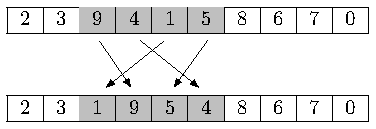
\includegraphics[width=0.9\linewidth]{include/graphs/mutation/scramble}}
		\caption{Scramble Mutation\label{fig:scramble}}
	\end{subfigure}
	\par\vskip12pt
	\begin{subfigure}{\linewidth}
		\centering 
		\fbox{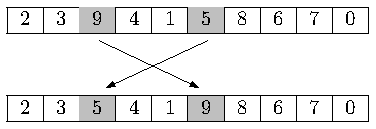
\includegraphics[width=0.9\linewidth]{include/graphs/mutation/swap}}
		\caption{Swap Mutation\label{fig:swap}}
	\end{subfigure}
	\caption{Two Types of Mutation Implemented}
\end{figure}

In such cases where generational fitness was not improving, 
scramble mutation was favoured $4:1$, the mutation rate was increased, crossover
rate was decreased $1:2$, severity of mutation\footnote{See
sub-sub-section~\ref{sssec:severity}.}
was increased fourfold, and survivor selection was done favouring the 
replacement operator, rather than $\mu + \lambda$.  
Replacement was favoured $3:1$ here because the new (more random) individuals 
may initially score lower (\ie higher Hamiltonian cycle distance) than existing 
individuals, however their varied genetic make-up could allow them to escape 
local minima more effectively. Such a 
scenario with $\mu + \lambda$ would result in many or all of the newer, less 
fit individuals immediately being removed from the population. When generational
fitness is improving, the two mutation types are favoured evenly, mutation rate is 
lowered back to $10\%$, crossover rate is reset to $90\%$, and survival
selection favours $\mu + \lambda$ $75\%$ of the time.

\subsubsection{Severity in the Scramble Mutation}\label{sssec:severity}
As the scramble mutation is now being used when randomness is desirable, the 
decision to capitalize on this operator's strength was made. The implementation
of this involves a mutation factor $f_m \in (0, 1)$. 

{\small\lstinputlisting[style=pycode]{include/snippets/scramble.py}}
\noindent A mutation threshold is then defined by ${t_m := f_m \cdot n}$. 
Two indices, |start_idx| and |end_idx|, both between $0$ and $n-1$, are 
selected at random from the individual. If |end_idx|${}-{}$|start_idx|${}< t_m$
then the algorithm chooses new indices until this requirement is satisfied.

Consequently, when high entropy is required a mutation factor can be chosen 
to enforce this (\eg if $f_m = 0.4$ then no less than $40\%$ of the individual
will be scrambled).

	\section{Results}
	%% BREAK LINES EVERY 80 CHARACTERS TO HELP GIT WITH MERGING
With the optimizations discussed in Section~\ref{ssec:precomputing}, 
pre-processing speeds increased dramatically from near-negligible time
to load the file to the times listed in Table~\ref{tab:precomputing}.
Note that there are only three entries per data set as pre-processing was 
done outside the |main()| function to save computation (\ie pre-processing
was done once for every 10 trials).
\begin{table}[h]
	\centering\small
	\def\arraystretch{1}
	\begin{tabular}{>{\bf}*4{c}} \hline 
		\textbf{Trial} & \textbf{Western Sahara} & \textbf{Uruguay} & \textbf{Canada} \\ \hline 
		1 & $112.342$ & $769.979$ & $31302.409$  \\
		2 & $110.887$ & $774.185$ & $30910.104$ \\
		3 & $110.485$ & $725.295$ & $30977.966$ \\ \hline 
	\end{tabular}
	\caption{Distance Pre-computation Times (ms)\label{tab:precomputing}}	
\end{table}
Execution of the GA was done with $5,000$ generations for each dataset 
with each generation taking approximately $400$, $1,200$, and $4,600$ 
milliseconds for Western Sahara, Uruguay, and Canada datasets, respectively.
For the smallest dataset, Western Sahara, $5,000$ proved to be a rather large 
number of iterations as the last generation with improved fitness hovers 
around $1,500$ (Table~\ref{tab:last-gen-tiny}). 
\begin{table}[H]
	\centering\small
	\tabcolsep=2pt
	\def\arraystretch{1}
	\begin{tabular}{*3{c}} \hline 
		\textbf{Trial} & \parbox{1.5cm}{\centering\bfseries Last\\Improve.} & \parbox{1.5cm}{\centering\bfseries Best\\Fitness} \\ \hline 
		1 & 1308 & 27620 \\
		2 & 4012 & 30664 \\
		3 & 2889 & 27768 \\
		4 & 3271 & 28513 \\
		5 & 4103 & 27768  \\
		6 & 3158 & 28202 \\
		7 & 1716 & 28202 \\
		8 & 1059 & 29154 \\
		9 & 1948 & 29098 \\
		10 & 2199 & 30048 \\
		11 & 4639 & 29177 \\
		12 & 1710 & 28039 \\
		13 & 839 & 27748 \\
		14 & 729 & 29686 \\
		15 & 597 & 29373 \\ \hline 
	\end{tabular}
	\begin{tabular}{*3{c}} \hline 
		\textbf{Trial} & \parbox{1.5cm}{\centering\bfseries Last\\Improve.} & \parbox{1.5cm}{\centering\bfseries Best\\Fitness} \\ \hline 
		16 & 1056 & 29337 \\
		17 &1407  & 27768 \\
		18 & 1686 & 28728 \\
		19 & 1078 & 28765 \\
		20 & 2371 & 28061 \\
		21 & 1534 & 28249 \\
		22 & 610 & 28735 \\
		23 & 4890 & 27620 \\
		24 & 2484 & 28249 \\
		25 & 803 & 29535 \\
		26 & 990 & 28231 \\
		27 & 1224 & 30709 \\
		28 & 810 & 30502 \\
		29 & 683 & 28222 \\
		30 & 4582 & 28755 \\ \hline 
	\end{tabular}
	\caption{Last Generation With Improvement (Western Sahara)\label{tab:last-gen-tiny}}
\end{table}
Consequently, Figure~\ref{fig:tiny-fitnesses} 
illustrates a plateau fairly early in the execution. This means that in 
some cases, similar results could be obtained much faster, with much
less computation. On the other hand, some trials have improvement 
as far as nearly $4,900$ generations into execution. Such trials sometimes
are the ones with the most optimal fitness (\eg trials $5$ and $23$
had improvement in generation $4,103$ and $4,890$, respectively 
and finished with best fitnesses of $27,768$ and $27,620$).
\begin{figure*}[h]
	\centering
	\fbox{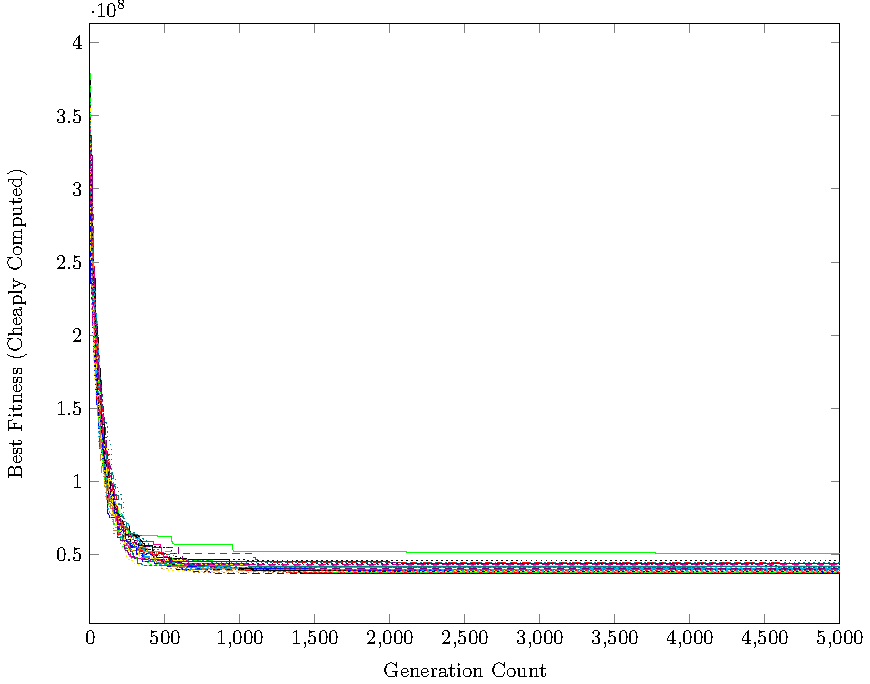
\includegraphics[width=0.65\linewidth]{include/graphs/fitness/tiny-fitnesses-lg}}
	\caption{Fitness Changes over $5,000$ Generations (Western Sahara)\label{fig:tiny-fitnesses}}
\end{figure*}
According to the University of Waterloo's Faculty of Mathematics, optimal fitness for this tour is $27,603$ \cite{sahara}. Therefore, several of the trials logged in Table~\ref{fig:tiny-fitnesses} show the algorithm's effectiveness in reaching near-optimal solutions. Given time to run more generations, optimal solutions should be achieved.

Uruguay, on the other hand, did not plateau in the same way that 
Western Sahara did (Figure~\ref{fig:med-fitnesses}).
\begin{table}[H]
	\centering\small
	\tabcolsep=2pt
	\def\arraystretch{1}
	\begin{tabular}{*3{c}} \hline 
		\textbf{Trial} & \parbox{1.5cm}{\centering\bfseries Last\\Improve.} & \parbox{1.5cm}{\centering\bfseries Best\\Fitness} \\ \hline 
		1 & 4995 & 682092 \\
		2 & 4987 & 686624 \\
		3 & 4991 & 675225 \\
		4 & 4993 & 675225 \\
		5 & 4974 & 685579  \\
		6 & 4990 & 673494 \\
		7 & 4996 & 689418 \\
		8 & 4996 & 678421 \\
		9 & 4995 & 659951 \\
		10 & 4999 & 687908 \\
		11 & 4987 & 680266 \\
		12 & 4988 & 699569 \\
		13 & 4998 & 702853 \\
		14 & 4993 & 696526 \\
		15 & 4995 & 701105 \\ \hline 
	\end{tabular}
	\begin{tabular}{*3{c}} \hline 
		\textbf{Trial} & \parbox{1.5cm}{\centering\bfseries Last\\Improve.} & \parbox{1.5cm}{\centering\bfseries Best\\Fitness} \\ \hline
		16 & 4993 & 687626 \\
		17 &4996  & 683809 \\
		18 & 4989 & 691854 \\
		19 & 4995 & 705421 \\
		20 & 4995 & 672055 \\
		21 & 4996 & 686104 \\
		22 & 4967 & 685925 \\
		23 & 4990 & 674031 \\
		24 & 4981 & 687605 \\
		25 & 4999 & 707432 \\
		26 & 4991 & 681644 \\
		27 & 4995 & 671644 \\
		28 & 4987 & 702787 \\
		29 & 4993 & 690934 \\
		30 & 4999 & 694009 \\ \hline 
	\end{tabular}
	\caption{Last Generation With Improvement (Uruguay)\label{tab:last-gen-med}}
\end{table}
\begin{figure*}[h]
	\centering
	\fbox{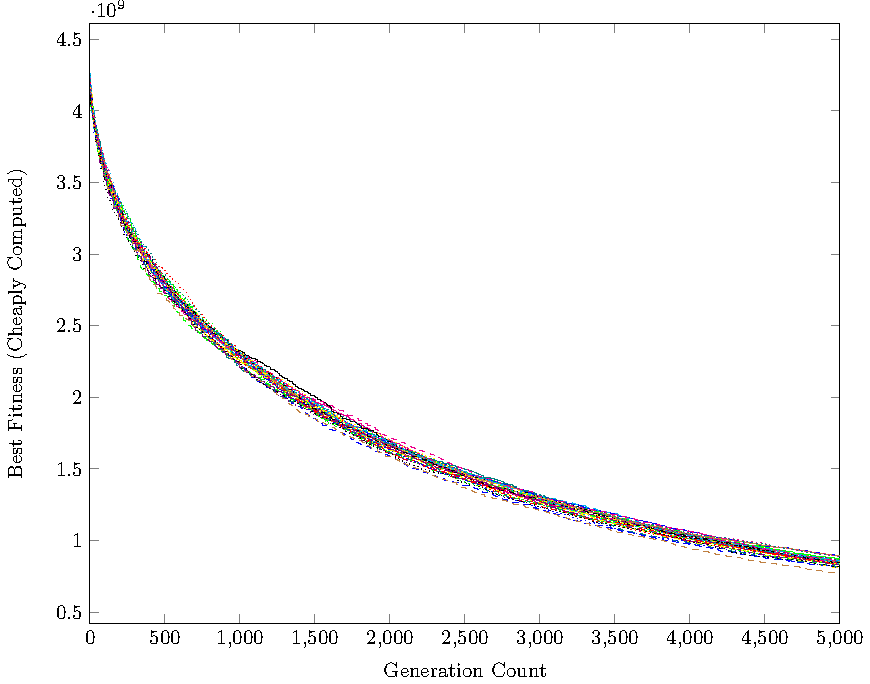
\includegraphics[width=0.65\linewidth]{include/graphs/fitness/med-fitnesses-lg}}
	\caption{Fitness Changes over $5,000$ Generations (Uruguay)\label{fig:med-fitnesses}}
\end{figure*}
This can be seen both by the way that Figure~\ref{fig:med-fitnesses}
maintains a relatively steep slope all the way to the last generation, 
as well as the high frequency of improvements above $4,980$ generations in
Table~\ref{tab:last-gen-med}.
Consequently, the algorithm, given more time to compute more generations,
should yield similar results as were demonstrated for Western Sahara.

Execution for the Canada dataset ran successfully for a number of trials,
however, due to the technique of running ten trials of the algorithm per execution,
technical errors mid-way through execution spoiled the data for all trials. 
	\section{Conclusion}
	%% BREAK LINES EVERY 80 CHARACTERS TO HELP GIT WITH MERGING
Results gathered from execution of the algorithm with the Western Sahara
dataset demonstrate the developed algorithm's efficacy in solving
the TSP. One improvement that the results from the Western Sahara
dataset indicate is a need for more effective local minima escaping 
techniques. Table~\ref{tab:last-gen-tiny} shows that in some cases
a high number of generations was required to achieve a near-optimal 
fitness, however Figure~\ref{fig:tiny-fitnesses} demonstrates a severe
plateau of best generational fitness around $500$ generations.

A more effective technique to escape local minima would reduce the 
number of generations with no improvement while still striving for 
near-optimal solutions.

While not as optimal, the results from the Uruguay dataset
do make sense and provide more useful information of where improvements
to the algorithm could be made. Extrapolation from 
Figure~\ref{fig:med-fitnesses} indicates that running more generations would likely 
result in a plateau of the best generational fitness much nearer the true
optimal solution. However, as execution for all datasets was done with
a constant population and mating pool size while the number of 
possible individuals grew at a rate of $n!$ for $n$ cities, future 
tests should be done with population and mating pool sizes that are not 
kept constant, but rather increase with the tour length. This would allow 
more variety in the population and hence could promote more diverse 
offspring, capable of escaping local minima faster and without 
reliance on severe mutation for randomness.
	\newpage
	\printbibliography
	\appendix
	\section{Source Code}
	%% BREAK LINES EVERY 80 CHARACTERS TO HELP GIT WITH MERGING
Source code and log files used in this report are available to the public
from the project's GitHub repository, located at 
\url{https://github.com/jwfh/cs3201-final-project}.
	\section{Computer Specifications}
	%% BREAK LINES EVERY 80 CHARACTERS TO HELP GIT WITH MERGING
\raggedbottom
As discussed in Section~\ref{ssec:hardware}, hardware limitations of the
computers used for algorithm execution were something that needed
to be considered and worked with in this project. Therefore, to 
facilitate an accurate and comprehensive report, hardware specifications
for all terminals used are included in this section. 


\subsection{Hosts Used}
A number of hosts belonging to Memorial's LabNet network were used to
run the GA developed for this report. These hosts are listed below.

\begin{verbatim}
   devastator.cs.mun.ca
   en2048ece03.engr.mun.ca
   en2048ece04.engr.mun.ca
   en2048ece05.engr.mun.ca
   en2048ece07.engr.mun.ca
   en2048ece12.engr.mun.ca
   laserbeak.cs.mun.ca
   overkill.cs.mun.ca
   pounce.cs.mun.ca
   starscream.cs.mun.ca
\end{verbatim}
Several other nodes were tested and not used due to lesser hardware 
capabilities.
\begin{verbatim}
   excalibur.cs.mun.ca
   excelsior.cs.mun.ca
   intrepid.cs.mun.ca
   reliant.cs.mun.ca
   valiant.cs.mun.ca
\end{verbatim}

\subsection{Processor Speed}
Specifications of the processor(s) in all nodes used for testing are 
included in Table~\ref{tab:cpu} on page~\pageref{tab:cpu}. 
\begin{table*}[ht]
	\centering\small
	\def\arraystretch{1.1}
	\begin{tabular}{lccccccc} \hline 
		\multirow{2}{*}{\bf Hostname} & \multirow{2}{*}{\bf Sockets} & \multirow{2}{*}{\parbox{1.75cm}{\centering\bf Cores per\\Socket}} & \multirow{2}{*}{\parbox{2cm}{\centering\bf Threads per Core}} & \multirow{2}{*}{\parbox{1.75cm}{\centering\bf CPU max.\\MHz}} & \multicolumn{3}{c}{\bf Cache}  \\ \cline{6-8}
		& & & & & {\bf L1} & {\bf L2} & {\bf L3} \\ \hline 
		|devastator| & 1 & 4 & 1 & 3800 & 32K & 256K & 6144K \\
		|en2048ece03| & 1 & 4 & 1 & 3600 & 32K & 256K & 6144K \\
		|en2048ece04| & 1 & 4 & 1 & 3600 & 32K & 256K & 6144K \\
		|en2048ece05| & 1 & 4 & 2 & 4000 & 32K & 256K & 8192K \\
		|en2048ece07| & 1 & 4 & 2 & 4000 & 32K & 256K & 8192K \\
		|en2048ece12| & 1 & 4 & 2 & 4000 & 32K & 256K & 8192K \\
		|excalibur| & 2 & 4 & 2 & 2668 & 32K & 256K & 8192K \\
		|excelsior| & 2 & 4 & 2 & 2668 & 32K & 256K & 8192K \\
		|laserbeak| & 1 & 4 & 1 & 3800 & 32K & 256K & 6144K \\
		|intrepid| & 2 & 4 & 2 & 2668 & 32K & 256K & 8192K \\
		|overkill| & 1 & 4 & 1 & 3800 & 32K & 256K & 6144K \\
		|pounce| & 1 & 4 & 1 & 3800 & 32K & 256K & 6144K \\
		|reliant| & 2 & 4 & 2 & 2668 & 32K & 256K & 8192K \\
		|starscream| & 1 & 4 & 1 & 3800 & 32K & 256K & 6144K \\ 
		|valiant| & 2 & 4 & 2 & 2668 & 32K & 256K & 8192K \\ \hline
	\end{tabular}
	\caption{Computer CPU Specifications\label{tab:cpu}}
\end{table*}

\subsection{Memory Specifications}
Due to conjecture made in Section~\ref{ssec:hardware} that one of the
limiting factors of the program execution time was random access 
memory (RAM) speed, an effort was made to retrieve these specifications
for the report. Unfortunately, due to system restrictions placed on 
LabNet computers, standard users do not have |sudo| privileges.
As a result, access to the |dmidecode| and |lshw| commands
needed to read information about system hardware is restricted.\label{sec:comp-specs}
\end{document}